\documentclass[article]{jss}

%% -- LaTeX packages and custom commands ---------------------------------------

%% recommended packages
\usepackage{thumbpdf,lmodern}

%% another package (only for this demo article)
\usepackage{framed}

%% new custom commands
\newcommand{\class}[1]{`\code{#1}'}
\newcommand{\fct}[1]{\code{#1()}}
\graphicspath{ {images/} }

%% For Sweave-based articles about R packages:
%% need no \usepackage{Sweave}



%% -- Article metainformation (author, title, ...) -----------------------------

%% - \author{} with primary affiliation
%% - \Plainauthor{} without affiliations
%% - Separate authors by \And or \AND (in \author) or by comma (in \Plainauthor).
%% - \AND starts a new line, \And does not.
\author{Konrad Stawiski\\ Medical University of Lodz
\And Marcin Kaszkowiak\\Medical University of Lodz
\And Damian Mikulski\\Medical Univeristy of Lodz
\AND Dipanjan Chowdhury\\Dana-Farber Cancer Institute
\And Wojciech Fendler\\Medical University of Lodz}
\Plainauthor{Konrad Stawiski, Marcin Kaszkowiak, Damian Mikulski, Dipanjan Chowdhury, Wojciech Fendler}

%% - \title{} in title case
%% - \Plaintitle{} without LaTeX markup (if any)
%% - \Shorttitle{} with LaTeX markup (if any), used as running title
\title{OmicSelector: \proglang{Docker}-based application and \proglang{R} package for biomarker signature selection from high-throughput omic experiments and deep learning model development.}
\Plaintitle{OmicSelector: Docker-based application and R package for biomarker signature selection from high-throughput omic experiments and deep learning model development.}
\Shorttitle{Biomarker selection and deep learning using OmicSelector.}

%% - \Abstract{} almost as usual
\Abstract{
  The crucial phase of modern biomarker discovery studies is a selection of most promising features from the results of high-throughput screening assays. Here, we present the OmicSelector - \proglang{Docker}-based web application and \proglang{R} package that facilitates the analysis of such experiments. OmicSelector provides a consistent and overfitting-resilient pipeline that integrates 94 feature selection approaches based on 25 distinct variable selection methods. It identifies and ranks the best feature sets, basing on 12 modeling algorithms (including GPU-based deep learning) with hyperparameter optimization in hold-out or cross-validation. OmicSelector provides classification performance metrics for proposed feature sets, which allow researchers to choose the overfitting-resistant biomarker set with the most significant diagnostic potential. Lastly, it allows for development, validation and implementation of deep learning feedforward neural networks (up to 3 hidden layers) on selected signature. Application performs extensive grid search of hyperparameters including balancing and preprocessing with additional autoencoders. The pipeline is applicable for selecting candidate circulating or tissue miRNAs, RNAs, methylation data, metabolites, or proteins. The tool is open-source and available at \url{https://biostat.umed.pl/OmicSelector/}.
}

%% - \Keywords{} with LaTeX markup, at least one required
%% - \Plainkeywords{} without LaTeX markup (if necessary)
%% - Should be comma-separated and in sentence case.
\Keywords{feature selection, biomarker, data-mining, next-generation sequencing, omics, deep learning, artificial neural network, \proglang{R}, \proglang{Docker}}
\Plainkeywords{feature selection, biomarker, data-mining, next-generation sequencing, omics, deep learning, artificial neural network, R, Docker}

%% - \Address{} of at least one author
%% - May contain multiple affiliations for each author
%%   (in extra lines, separated by \emph{and}\\).
%% - May contain multiple authors for the same affiliation
%%   (in the same first line, separated by comma).
\Address{
  Konrad Stawiski, M.D.\\
  Department of Biostatistics and Translational Medicine\\
  Medical University of Lodz\\
  Mazowiecka 15\\
  92-215 Lodz, Poland\\
  E-mail: \email{konrad.stawiski@umed.lodz.pl}, \email{konrad@konsta.com.pl}\\
  URL: \url{https://biostat.umed.pl/person/?surname=stawiski}, \url{https://konsta.com.pl}
}

\begin{document}


%% -- Introduction -------------------------------------------------------------

%% - In principle "as usual".
%% - But should typically have some discussion of both _software_ and _methods_.
%% - Use \proglang{}, \pkg{}, and \code{} markup throughout the manuscript.
%% - If such markup is in (sub)section titles, a plain text version has to be
%%   added as well.
%% - All software mentioned should be properly \cite-d.
%% - All abbreviations should be introduced.
%% - Unless the expansions of abbreviations are proper names (like "Journal
%%   of Statistical Software" above) they should be in sentence case (like
%%   "generalized linear models" below).

\section[Introduction]{Introduction} \label{sec:intro}

Broad-scale treatment personalization is one of the most significant modern medicine challenges, requiring accurate and cost-effective diagnostic tests. Such methods rely heavily on biomarkers, which are usually discovered using omic techniques. Although high-throughput experiments enable us to gather the biological measurements of an extensive amount of biomarker candidates, translating the results to the clinical bedside remains troublesome.

The typical biomarker study comprises of discovery and validation phases. (\cite{Goossens2015}) In the former, high-throughput screening is usually performed to measure the values of multiple features. Those are further assessed to determine their diagnostic potential. In the validation phase, only selected variables are measured, typically in a new set of samples, with a cheaper and/or more accessible method.
Our team has been working on microRNA (miRNA) biomarkers for radiation (\cite{Dinh2016b}) and cancer (\cite{Elias2017c}), but trouble with the reproducibility of selected biomarker performance (\cite{Acharya2015,Fendler2017,Maachowska2020}) or reference identification (\cite{Pagacz2020}). Similar challenges, caused by bias and overfitting, hindered the attempts of other groups to develop validated, efficient omic-driven biomarkers. (\cite{Dobbin2016})

Cohorts used in the discovery phase are usually small due to the high cost of high-throughput assays, which makes the experiments vulnerable to overfitting and results in false-positive biomarker candidates that fail in external validation. (\cite{Smialowski2009}) For example, a recent review of serum miRNA biomarkers for pancreatic cancer (\cite{Xue2019}) highlights how various miRNA sets are chosen in different studies, with each study reporting unrealistically optimistic results. Thus, correct and overfitting-resistant feature selection is critical in biomarker studies.

\begin{figure}[h!]
  \caption{\emph{\textbf{The pipeline of OmicSelector analysis.} Abbreviations: PCA - principal component analysis, BH - Benjamini-Hochberg procedure, SMOTE/ROSE - data balancing methods explained in the main text.}}\label{fig:1}
  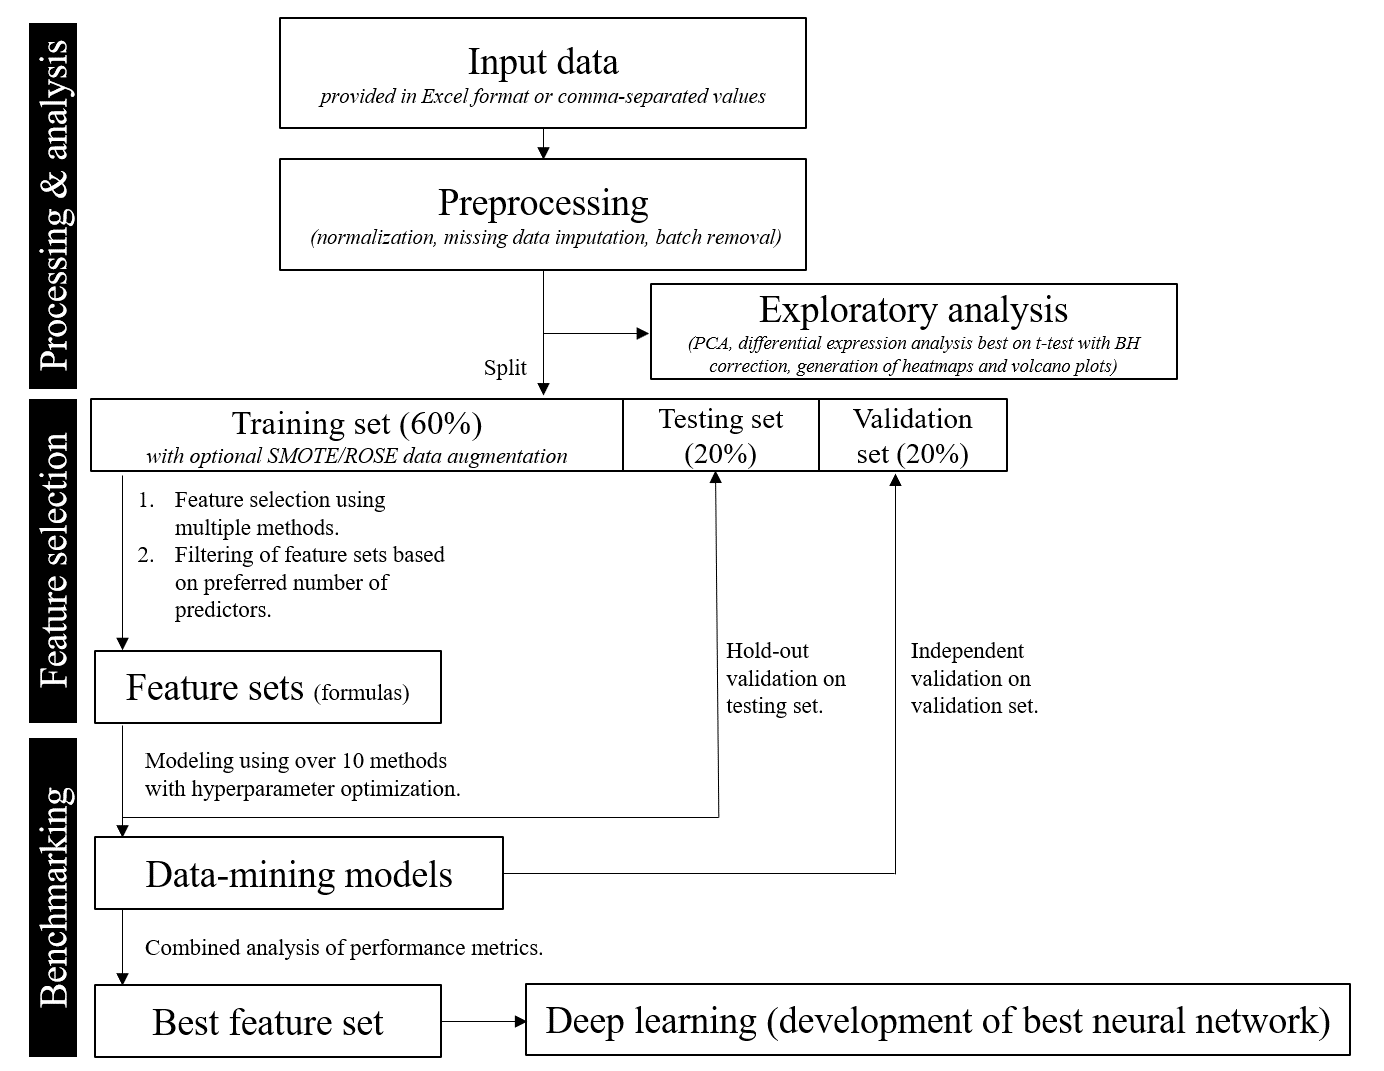
\includegraphics[width=1\textwidth]{figure1.png}
\end{figure}

In this paper, we try to tackle this problem by designing software for systematic, overfitting-resistant, and informative feature selection. The analytical steps of our package entail (Figure \ref{fig:1}): splitting of the dataset into training, testing and validation sets, differential expression analysis and performing up to 94 different feature selection procedures on the training set. Feature sets (formulas) are further validated by training 12 models of various architectures with hyperparameter optimization based on hold-out- or cross-validation. Our toolset enables the users to make an informed decision about the most appropriate feature selection method and informs them about their predictive abilities using different modeling approaches. Finally, as the most flexible method, users are able to train and implement final deep feedforward neural network (up to 3 hidden layers, with or without autoencoders; grid search of hyperparameters) for classification (diagnostic) problem.




%% -- Manuscript ---------------------------------------------------------------

%% - In principle "as usual" again.
%% - When using equations (e.g., {equation}, {eqnarray}, {align}, etc.
%%   avoid empty lines before and after the equation (which would signal a new
%%   paragraph.
%% - When describing longer chunks of code that are _not_ meant for execution
%%   (e.g., a function synopsis or list of arguments), the environment {Code}
%%   is recommended. Alternatively, a plain {verbatim} can also be used.
%%   (For executed code see the next section.)

\section{Implementation} \label{sec:implementation}

\begin{Schunk}
\begin{Sinput}
R> library(OmicSelector)
R> sessionInfo()
\end{Sinput}
\begin{Soutput}
R version 4.0.3 (2020-10-10)
Platform: x86_64-pc-linux-gnu (64-bit)
Running under: Ubuntu 18.04.5 LTS

Matrix products: default
BLAS:   /usr/lib/x86_64-linux-gnu/openblas/libblas.so.3
LAPACK: /usr/lib/x86_64-linux-gnu/libopenblasp-r0.2.20.so

locale:
 [1] LC_CTYPE=en_US.UTF-8       LC_NUMERIC=C              
 [3] LC_TIME=en_US.UTF-8        LC_COLLATE=en_US.UTF-8    
 [5] LC_MONETARY=en_US.UTF-8    LC_MESSAGES=en_US.UTF-8   
 [7] LC_PAPER=en_US.UTF-8       LC_NAME=C                 
 [9] LC_ADDRESS=C               LC_TELEPHONE=C            
[11] LC_MEASUREMENT=en_US.UTF-8 LC_IDENTIFICATION=C       

attached base packages:
[1] stats     graphics  grDevices utils     datasets  methods  
[7] base     

other attached packages:
[1] OmicSelector_1.0.0 MASS_7.3-53       

loaded via a namespace (and not attached):
[1] compiler_4.0.3    snow_0.4-3        parallel_4.0.3   
[4] tools_4.0.3       codetools_0.2-18  doParallel_1.0.16
[7] iterators_1.0.13  foreach_1.5.1    
\end{Soutput}
\end{Schunk}

\begin{tabular}{|p{0.2in}|p{2.0in}|p{3.9in}|} \hline
\textbf{N} & \textbf{ID} & \textbf{Description} \\ \hline
1 & all [1] & Get all features (all features staring with 'hsa' in the name). We assume that the most frequent application of the pipeline will be for human-related expression measurements. \\ \hline
2 & sig [2]sigtop [2]sigtopBonf[ 2]sigtopHolm [2]topFC [2]sig\_SMOTE [2]sigtop\_SMOTE [2]sigtopBonf\_SMOTE [2]sigtopHolm\_SMOTE [2]topFC\_SMOTE [2] & Selects features significantly differently expressed between classes by performing unpaired t-test with and without correction for multiple testing.We get:~\textbf{sig}~- all significant (adjusted p-value less or equal to 0.05) miRNAs with comparison using unpaired t-test and after the Benjamini-Hochberg procedure;~\textbf{sigtop}~-~sig limited only to the number of features preffered by an user (selecting top after sorting by p-value),~\textbf{sigtopBonf}~- uses Bonferroni instead of BH correction,~\textbf{sigtopHolm}~- uses Holm--Bonferroni instead of BH correction,~\textbf{topFC}~- selects prefered number of features based on decreasing absolute value of fold change in differential analysis. \\ \hline
3 & fcsig [3]fcsig\_SMOTE [3] & Features significantly differently expressed with absolute log2FC greater than 1. (Thus, features significantly up- or down-regulated in the higher magnitudes)  \\ \hline
4 & cfs [4]cfs\_SMOTE [4]cfs\_sig [4]cfs\_SMOTE\_sig [4] & Correlation-based feature selection~(CFS) - a heuristic algorithm selecting features that are highly correlated with class (binary) and lowly correlated with one another. It explores a search space in best-first manner, until stopping criteria are met. \\ \hline
5 & classloop [5]\newline classloop\_SMOTE [6]\newline classloop\_sig [7]\newline classloop\_SMOTE\_sig [8] & Classifier loop - performs multiple classification procedures using various algorithms (with embedded feature ranking) and various performance metrices. Final feature selection is done by combining the results. Modeling methods used: support vector machines, linear discriminant a nalysis, random forest and nearest shrunken centroid. Features are selected based on the AUC ROC and assessed in k-fold cross-validation according to the~documentation.  \\ \hline
6 & fcfs [9]\newline fcfs\_SMOTE [10]\newline fcfs\_sig [11]\newline fcfs\_SMOTE\_sig [12] & An algorithm similar to CFS, though exploring search space in greedy forward search manner (adding one, most attractive, feature at the time, until such addition does not improve set's overall quality). Based on~Wang et al. 2005~and documented~here. \\ \hline
7 & fwrap [13]\newline fwrap\_SMOTE [14]\newline fwrap\_sig [15]\newline fwrap\_SMOTE\_sig [16] & A decision tree algorithm and forward search strategy documented~here. \\ \hline
8 & AUC\_MDL [17]\newline AUC\_MDL\_SMOTE [20]\newline AUC\_MDL\_sig [23]\newline AUC\_MDL\_SMOTE\_sig [26] & Feature ranking based on ROC AUC and minimal description length (MDL) discretization algorithm documented~here\underbar{.} \\ \hline
9 & SU\_MDL [18]\newline SU\_MDL\_SMOTE [21]\newline SU\_MDL\_sig [24]\newline SU\_MDL\_SMOTE\_sig [27] & Feature ranking based on symmetrical uncertainty and minimal description length (MDL) discretization algorithm documented~here. \\ \hline
10 & CorrSF\_MDL [19]\newline CorrSF\_MDL\_SMOTE [22]\newline CorrSF\_MDL\_sig [25]\newline CorrSF\_MDL\_SMOTE\_sig [28] & Feature ranking based on CFS algorithm with forward search and minimal description length (MDL) discretization algorithm documented~here. \\ \hline
11 & bounceR-full [29]\newline bounceR-full\_SMOTE [30]\newline bounceR-full\_sig [31]\newline bounceR-full\_SMOTE\_sig [32]bounceR-stability [29]\newline bounceR-stability\_SMOTE [30]\newline bounceR-stability\_SIG [31]\newline bounceR-stability\_SMOTE\_sig [32] & A component-wise-boosting-based algorithm selecting optimal features in multiple iterations of single feature-models construction. See the source~here.~\textbf{bounceR-stability}~gets the most stable features. Wrapper methods implemented here leverage component-wise boosting as a weak learners. \\ \hline
12 & RandomForestRFE [33]\newline RandomForestRFE\_SMOTE [34]\newline RandomForestRFE\_sig [35]\newline RandomForestRFE\_SMOTE\_sig [36] & Recursively eliminates features from the feature space based on ranking from Random Forrest classifier (retrained with resampling after each elimination). Details are available~here. \\ \hline
13 & GeneticAlgorithmRF [37]\newline GeneticAlgorithmRF\_SMOTE [38]\newline GeneticAlgorithmRF\_sig [39]\newline GeneticAlgorithmRF\_SMOTE\_sig [40] & Uses genetic algorithm principle to search for optimal subset of the feature space. This uses internally implemented random forest model and 10-fold cross validation to assess performance of the "chromosomes" in each generation. Details are available~here. \\ \hline
14 & SimulatedAnnealingRF [41]\newline SimulatedAnnealingRF\_SMOTE [42]\newline SimulatedAnnealingRF\_sig [43]\newline SimulatedAnnealingRF\_SMOTE\_sig [44] & Explores a feature space by randomly modifying a given feature subset and evaluating classification performance to check whether changes were beneficial. It is is a global search method that makes small random changes (i.e. perturbations) to an initial candidate solution. In this method also random forest is used as a model for evaluation. Details are available~here. \\ \hline
15 & Boruta [45]\newline Boruta\_SMOTE [46] & Utilizes random forrest algorithm to iteratively remove features proved to be less relevant than random variables. Details are available in paper by~Kursa et al. 2010~or~this blog post. Performed only on features significantly differently expressed between groups  \\ \hline
16 & spFSR [47]\newline spFSR\_SMOTE [48] & Feature selection and ranking by simultaneous perturbation stochastic approximation. This is an algorithm based on pseudo-gradient descent stochastic optimisation with Barzilai-Borwein method for step size and gradient estimation optimization. Details are available in paper by~Zeren et al. 2018. \\ \hline
17 & varSelRF [49]varSelRF\_SMOTE [49] & varSelRF - recursively eliminates features using random forest feature scores, seeking to minimize out-of-bag classification error. Details are available in paper by~D\'{i}az-Uriarte et al. 2006\underbar{.} \\ \hline
18 & Wx [50]Wx\_SMOTE [50] & Deep neural network-based (deep learning) feature (gene) selection algorithm.~We use 2 hidden layers with 16 hidden neurons.~Details are available in paper by~Park et al. 2019.  \\ \hline
19 & Mystepwise\_glm\_binomial [51]\newline Mystepwise\_glm\_binomial\_sig [51]\newline Mystepwise\_glm\_binomial\_SMOTE [52]\newline Mystepwise\_ glm\_binomial\_SMOTE\_sig [52] & Stepwise variable selection procedure (with iterations between the 'forward' and 'backward' steps) for generalized linear models with logit link function (i.e. logistic regression). We use p=0.05 as a threshold for both entry (SLE) and stay (SLS). Details are available~here\underbar{.} \\ \hline
20 & stepAIC [53]stepAIC\_sig [53]\newline stepAIC\_SMOTE [54]\newline stepAIC\_SMOTE\_sig [54] & Stepwise feature selection using model's (logistic regression based) AIC (Akaike Information Criterion) as a metric. Details are available~here. \\ \hline
21 & iteratedRFECV [55]iteratedRFETest [55] & Runs multiple iterations of Recursive Feature Elimination algorithm (details) with different initial random state. The results are then aggregated using ensemble voting procedure. Utilizes either cross-validation or test set for model performance evaluation (suffixes `\_CV' and `\_Test' respectively); watch out for bias!). See the source~here. \\ \hline
 & iteratedRFECV\_SMOTE [56] iteratedRFETest\_SMOTE [56] &  \\ \hline
22 & LASSO [57]LASSO\_SMOTE [57] & Feature selection based on LASSO (Least Absolute Shrinkage and Selection Operator) model with alpha = 1 - penalized with L1-norm; with 10-fold cross-validation. See the source~here.  \\ \hline
23 & ElasticNet [58]ElasticNet\_SMOTE [58] & Feature selection based on elastic net with the alpha value tuned through a line search. See the source~here.  \\ \hline
24 & stepLDA [59]\newline stepLDA\_SMOTE [59] & Forward/backward variable selection (both directions) for linear discriminant analysis. See the source~here. \\ \hline
25 & feseR\_filter.corr [60]\newline feseR\_filter.corr\_SMOTE [60]\newline feseR\_gain.inf [60]\newline feseR\_gain.inf\_SMOTE [60]\newline feseR\_matrix.corr [60]\newline feseR\_matrix.corr\_SMOTE [60]\newline feseR\_combineFS\_RF [60] feseR\_combineFS\_RF\_SMOTE [60] & Set of feature selection methods embeded in feseR package published by Perez-Rivelor et al. All default parameters are used, but mincorr package version is set to 0.2. See the paper~here.  \\ \hline
\end{tabular}


%% -- Illustrations ------------------------------------------------------------

%% - Virtually all JSS manuscripts list source code along with the generated
%%   output. The style files provide dedicated environments for this.
%% - In R, the environments {Sinput} and {Soutput} - as produced by Sweave() or
%%   or knitr using the render_sweave() hook - are used (without the need to
%%   load Sweave.sty).
%% - Equivalently, {CodeInput} and {CodeOutput} can be used.
%% - The code input should use "the usual" command prompt in the respective
%%   software system.
%% - For R code, the prompt "R> " should be used with "+  " as the
%%   continuation prompt.
%% - Comments within the code chunks should be avoided - these should be made
%%   within the regular LaTeX text.

\section{Illustrations} \label{sec:illustrations}

For a simple illustration of basic Poisson and NB count regression the
\code{quine} data from the \pkg{MASS} package is used. This provides the number
of \code{Days} that children were absent from school in Australia in a
particular year, along with several covariates that can be employed as regressors.
The data can be loaded by
%
\begin{Schunk}
\begin{Sinput}
R> data("quine", package = "MASS")
\end{Sinput}
\end{Schunk}
%
and a basic frequency distribution of the response variable is displayed in
Figure~\ref{fig:quine}.

\begin{leftbar}
For code input and output, the style files provide dedicated environments.
Either the ``agnostic'' \verb|{CodeInput}| and \verb|{CodeOutput}| can be used
or, equivalently, the environments \verb|{Sinput}| and \verb|{Soutput}| as
produced by \fct{Sweave} or \pkg{knitr} when using the \code{render_sweave()}
hook. Please make sure that all code is properly spaced, e.g., using
\code{y = a + b * x} and \emph{not} \code{y=a+b*x}. Moreover, code input should
use ``the usual'' command prompt in the respective software system. For
\proglang{R} code, the prompt \code{"R> "} should be used with \code{"+  "} as
the continuation prompt. Generally, comments within the code chunks should be
avoided -- and made in the regular {\LaTeX} text instead. Finally, empty lines
before and after code input/output should be avoided (see above).
\end{leftbar}

\begin{figure}[t!]
\centering
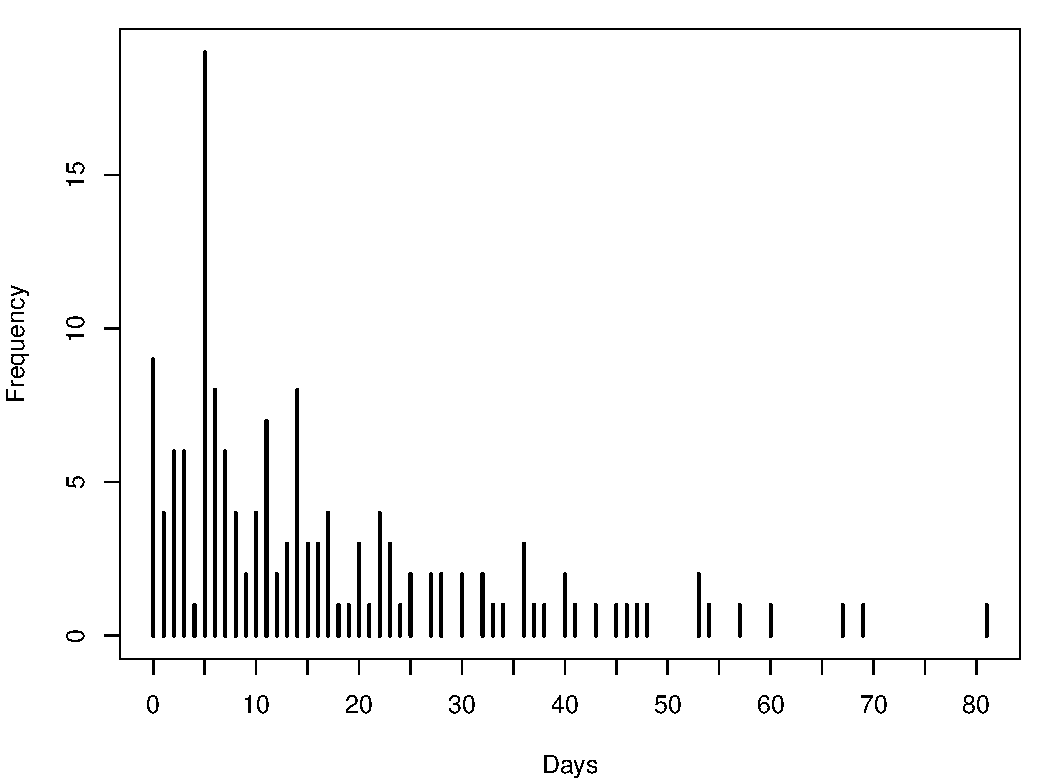
\includegraphics{article-visualization}
\caption{\label{fig:quine} Frequency distribution for number of days absent
from school.}
\end{figure}

As a first model for the \code{quine} data, we fit the basic Poisson regression
model. (Note that JSS prefers when the second line of code is indented by two
spaces.)
%
\begin{Schunk}
\begin{Sinput}
R> m_pois <- glm(Days ~ (Eth + Sex + Age + Lrn)^2, data = quine,
+    family = poisson)
\end{Sinput}
\end{Schunk}
%
To account for potential overdispersion we also consider a negative binomial
GLM.
%
\begin{Schunk}
\begin{Sinput}
R> library("MASS")
R> m_nbin <- glm.nb(Days ~ (Eth + Sex + Age + Lrn)^2, data = quine)
\end{Sinput}
\end{Schunk}
%
In a comparison with the BIC the latter model is clearly preferred.
%
\begin{Schunk}
\begin{Sinput}
R> BIC(m_pois, m_nbin)
\end{Sinput}
\begin{Soutput}
       df      BIC
m_pois 18 2046.851
m_nbin 19 1157.235
\end{Soutput}
\end{Schunk}
%
Hence, the full summary of that model is shown below.
%
\begin{Schunk}
\begin{Sinput}
R> summary(m_nbin)
\end{Sinput}
\begin{Soutput}
Call:
glm.nb(formula = Days ~ (Eth + Sex + Age + Lrn)^2, data = quine, 
    init.theta = 1.60364105, link = log)

Deviance Residuals: 
    Min       1Q   Median       3Q      Max  
-3.0857  -0.8306  -0.2620   0.4282   2.0898  

Coefficients: (1 not defined because of singularities)
            Estimate Std. Error z value Pr(>|z|)    
(Intercept)  3.00155    0.33709   8.904  < 2e-16 ***
EthN        -0.24591    0.39135  -0.628  0.52977    
SexM        -0.77181    0.38021  -2.030  0.04236 *  
AgeF1       -0.02546    0.41615  -0.061  0.95121    
AgeF2       -0.54884    0.54393  -1.009  0.31296    
AgeF3       -0.25735    0.40558  -0.635  0.52574    
LrnSL        0.38919    0.48421   0.804  0.42153    
EthN:SexM    0.36240    0.29430   1.231  0.21818    
EthN:AgeF1  -0.70000    0.43646  -1.604  0.10876    
EthN:AgeF2  -1.23283    0.42962  -2.870  0.00411 ** 
EthN:AgeF3   0.04721    0.44883   0.105  0.91622    
EthN:LrnSL   0.06847    0.34040   0.201  0.84059    
SexM:AgeF1   0.02257    0.47360   0.048  0.96198    
SexM:AgeF2   1.55330    0.51325   3.026  0.00247 ** 
SexM:AgeF3   1.25227    0.45539   2.750  0.00596 ** 
SexM:LrnSL   0.07187    0.40805   0.176  0.86019    
AgeF1:LrnSL -0.43101    0.47948  -0.899  0.36870    
AgeF2:LrnSL  0.52074    0.48567   1.072  0.28363    
AgeF3:LrnSL       NA         NA      NA       NA    
---
Signif. codes:  0 '***' 0.001 '**' 0.01 '*' 0.05 '.' 0.1 ' ' 1

(Dispersion parameter for Negative Binomial(1.6036) family taken to be 1)

    Null deviance: 235.23  on 145  degrees of freedom
Residual deviance: 167.53  on 128  degrees of freedom
AIC: 1100.5

Number of Fisher Scoring iterations: 1


              Theta:  1.604 
          Std. Err.:  0.214 

 2 x log-likelihood:  -1062.546 
\end{Soutput}
\end{Schunk}



%% -- Summary/conclusions/discussion -------------------------------------------

\section{Summary and discussion} \label{sec:summary}

\begin{leftbar}
As usual \dots
\end{leftbar}


%% -- Optional special unnumbered sections -------------------------------------

\section*{Computational details}

\begin{leftbar}
If necessary or useful, information about certain computational details
such as version numbers, operating systems, or compilers could be included
in an unnumbered section. Also, auxiliary packages (say, for visualizations,
maps, tables, \dots) that are not cited in the main text can be credited here.
\end{leftbar}

The results in this paper were obtained using
\proglang{R}~4.0.3 with the
\pkg{MASS}~7.3.53 package. \proglang{R} itself
and all packages used are available from the Comprehensive
\proglang{R} Archive Network (CRAN) at
\url{https://CRAN.R-project.org/}.


\section*{Acknowledgments}

\begin{leftbar}
All acknowledgments (note the AE spelling) should be collected in this
unnumbered section before the references. It may contain the usual information
about funding and feedback from colleagues/reviewers/etc. Furthermore,
information such as relative contributions of the authors may be added here
(if any).
\end{leftbar}


%% -- Bibliography -------------------------------------------------------------
%% - References need to be provided in a .bib BibTeX database.
%% - All references should be made with \cite, \citet, \citep, \citealp etc.
%%   (and never hard-coded). See the FAQ for details.
%% - JSS-specific markup (\proglang, \pkg, \code) should be used in the .bib.
%% - Titles in the .bib should be in title case.
%% - DOIs should be included where available.

\bibliography{refs}


%% -- Appendix (if any) --------------------------------------------------------
%% - After the bibliography with page break.
%% - With proper section titles and _not_ just "Appendix".

\newpage

\begin{appendix}

\section{More technical details} \label{app:technical}

\begin{leftbar}
Appendices can be included after the bibliography (with a page break). Each
section within the appendix should have a proper section title (rather than
just \emph{Appendix}).

For more technical style details, please check out JSS's style FAQ at
\url{https://www.jstatsoft.org/pages/view/style#frequently-asked-questions}
which includes the following topics:
\begin{itemize}
  \item Title vs.\ sentence case.
  \item Graphics formatting.
  \item Naming conventions.
  \item Turning JSS manuscripts into \proglang{R} package vignettes.
  \item Trouble shooting.
  \item Many other potentially helpful details\dots
\end{itemize}
\end{leftbar}


\section[Using BibTeX]{Using \textsc{Bib}{\TeX}} \label{app:bibtex}

\begin{leftbar}
References need to be provided in a \textsc{Bib}{\TeX} file (\code{.bib}). All
references should be made with \verb|\cite|, \verb|\citet|, \verb|\citep|,
\verb|\citealp| etc.\ (and never hard-coded). This commands yield different
formats of author-year citations and allow to include additional details (e.g.,
pages, chapters, \dots) in brackets. In case you are not familiar with these
commands see the JSS style FAQ for details.

Cleaning up \textsc{Bib}{\TeX} files is a somewhat tedious task -- especially
when acquiring the entries automatically from mixed online sources. However,
it is important that informations are complete and presented in a consistent
style to avoid confusions. JSS requires the following format.
\begin{itemize}
  \item JSS-specific markup (\verb|\proglang|, \verb|\pkg|, \verb|\code|) should
    be used in the references.
  \item Titles should be in title case.
  \item Journal titles should not be abbreviated and in title case.
  \item DOIs should be included where available.
  \item Software should be properly cited as well. For \proglang{R} packages
    \code{citation("pkgname")} typically provides a good starting point.
\end{itemize}
\end{leftbar}

\end{appendix}

%% -----------------------------------------------------------------------------


\end{document}
